\documentclass{article}
\usepackage{graphicx}
\usepackage{amsthm}
\usepackage{amsmath}
\usepackage{mathtools}
\usepackage{amssymb}
\usepackage{tikz-cd}
\usepackage{etoolbox}
\usepackage[]{algorithm2e}
\usepackage[section]{placeins}


\usepackage{geometry}
 \geometry{
 a4paper,
 total={170mm,257mm},
 left=20mm,
 top=20mm,
 }

\let\oldproofname=\proofname
\renewcommand\proofname{\bf{\oldproofname}}
\renewcommand\qedsymbol{$\blacksquare$}

\theoremstyle{definition}
\newtheorem{thm}{Theorem}
\newtheorem{lemma}{Lemma}
\newtheorem{defn}{Definition}[section]

\newcommand{\notimplies}{%
  \mathrel{{\ooalign{\hidewidth$\not\phantom{=}$\hidewidth\cr$\implies$}}}}

\newcommand{\cat}{
  \mathbf
}
\newcommand{\domain}[1]{
  \mathrm{dom}(#1)
}
\newcommand{\codomain}[1]{
  \mathrm{cod}(#1)
}
\newcommand{\idarrow}[1][]{
  \mathrm{1}_{#1}
}

\AtBeginEnvironment{quote}{\singlespacing\small}

\setlength{\parskip}{1em}
\setlength{\parindent}{2em}


\begin{document}

\title{Casper Research: \\ A Specification of Casper the Friendly Ghost \\ A ``Correct-by-Construction'' Blockchain Consensus Protocol \\ DRAFT v0.1 \\}
\author{Vlad Zamfir}
\maketitle

\begin{abstract}
We present a specification and limited experimental observations of a blockchain-based consensus protocol, ``Casper the Friendly Ghost.''

The protocol uses an adaptation of Y.\ Jompolovsky and A.\ Zohar's Greedy Heaviest Observed Sub-tree (GHOST) as a ``fork-choice rule.'' It is able to finalize/decide on blocks with asynchronous and Byzantine fault tolerant consensus safety. It allows blocks to be finalized while the network operates with the network overhead of the Bitcoin blockchain, with each node receiving $\mathcal{O}(1)$ messages/block. This is in contrast to the $\mathcal{O}(N)$ traditionally required for Byzantine fault tolerant state machine replication.

For pedagogical reasons, we first specify a binary consensus protocol (which decides on a bit, $0$ or $1$). This binary consensus protocol satisfies the same consensus safety proof as the blockchain consensus protocol and is therefore very similar to the blockchain consensus protocol.

\end{abstract}

\section{Introduction}

Consensus protocols are used by nodes in distributed systems to decide on the same consensus values, or on the same list of inputs to a replicated state machine. This is a challenging problem due to both network latency and the presence of faulty nodes. Arbitrary network latency, for example, means that nodes recieve distinct sets of messages, while the messages that they each receive may arrive in different orders. Faulty nodes may go offline, or they may behave in an arbitrary manner.

There are, roughly speaking, two broad classes of consensus protocols known today. One we refer to as ``traditional consensus.'' This class has its ``genetic roots'' in Paxos and multi-Paxos[CITE], and in the ``traditional'' consensus protocol research from the 80s and 90s[CITE]. The other we refer to as ``blockchain consensus.'' These are protocols that have their roots in the Bitcoin blockchain and Satoshi Nakamoto's whitepaper[CITE]. We first discuss the differences between these classes of protocols. Then we give an overview of the safety proof that the protocols found in this document satisfy, and finally we present the specifications of the protocols at hand.

\subsection{Comparing Traditional Consensus to Blockchain Consensus}

Traditional consensus protocols (such as multi-Paxos and pbft) are notoriously difficult to understand[CITE (http://paxos.systems/)]. Blockchain consensus protocols, on the other hand, are much more accessible. This difference comes at least in part from the relative simplicity of Bitcoin's specification[CITE].

In the context of state machine replication, traditional protocols decide (with irrevocable finality) on one ``block'' of state transitions/transactions to add to the shared operation log at a time. To decide on a block, a node must receive $\mathcal{O}(N)$ messages, where $N$ is the number of consensus-forming nodes.

Blockchain consensus protocols like Bitcoin do not finalize/decide on one block at a time. In fact, the Bitcoin blockchain in particular does not make ``finalized decisions'' at all; blocks are ``orphaned'' if/when they are not in the highest total difficulty chain. However, if the miners are able to mine on the same blockchain, then the blocks that get deep enough into the blockchain won't be reverted (``orphaned''). A block's depth in the blockchain therefore serves as a proxy for finalization. In the average case for blockchain consensus protocols, each node only requires approximately one message, $\mathcal{O}(1)$, for every block.

Traditional consensus protocol research has focused on producing protocols that are asynchronously safe (i.e.\ blocks won't be reverted due to arbitrary timing of future events) and live in asynchrony (or partial synchrony) (i.e.\ nodes eventually decide on new blocks). On the other hand, the Bitcoin blockchain is not safe or live in an asynchonous network but is safe and live (for unknown block-depth or ``confirmation count'') in a ``partially synchronous network.''

Traditional Byzantine fault tolerant consensus protocols have precisely stated Byzantine fault tolerance numbers (often can tolerate less than a third Byzantine faults, or up to $t$ faults when there are $3t + 1$ nodes)[CITE]. On the other hand, it is less clear exactly how many faults (measured as a proportion of hashrate) the Bitcoin blockchain protocol can tolerate[CITE].

\subsection{Overview of the Work Presented}

We give the specification of a consensus protocol, ``Casper the Friendly Ghost,'' which has both the low overhead of blockchain consensus protocols and the asynchronous Byzantine fault tolerant safety normally associated with traditional consensus protocols. However, before we share the blockchain consensus protocol, we give the specification of a binary consensus protocol (which chooses between $0$ and $1$ with asynchronous, Byzantine fault tolerant safety).

Understanding the binary consensus protocol makes it much easier to understand the blockchain consensus protocol; the protocols are remarkably similar. They are so similar because they are both ``generated'' in order to satisfy the same consensus safety proof.

This process for choosing the protocol specification is not specified or justified here, but rather in another, more abstract, paper[CITE]. This paper lacks information about \emph{why exactly} certain choices were made or \emph{how exactly} certain claims are proven. Even without the full scope of the ``process paper,'' our aim is to provide the reader with clear intuitions about why/how the blockchain protocol works. We therefore give a high level sketch of the safety proof which these protocols satisfy. Then, we present the promised protocols.

\subsection{Consensus Safety Proof}

Each of the protocols presented satisfies the same consensus safety proof. (And indeed, any consensus protocol generated by the correct-by-construction process\footnote{See our related paper -- PAPER} satisfies the same proof.)

We will assume that nodes running the consensus protocol have (local) states in $\Sigma$. These states have directional paths called ``protocol executions'' or ``protocol state transitions'' between them. We will write $\sigma \to \sigma'$ if there is an execution from $\sigma$ to $\sigma'$. Additionally, the paths are composable, so if $\sigma \to \sigma'$ and $\sigma' \to \sigma''$, then there is also an execution $\sigma \to \sigma''$.

The proof refers to an ``estimator,'' which maps protocol states to propositions about the consensus. In the binary consensus, the estimator maps protocol states to $0$ or $1$. In the blockchain consensus, on the other hand, the estimator maps from protocol states to a blockchain (functioning as our ``fork choice'').

An estimate in the binary consensus ($0$ or $1$) is said to be ``safe'' (have ``estimate safety'') for a particular protocol state if it is returned by the estimator on all future protocol states\footnote{Meaning, all states accessible from that state through any valid protocol execution}. In the blockchain consensus, a block is said to be ``safe'' for a particular protocol state if it is also in the fork choice for all future protocol states.

The consensus safety proof shows that decisions on safe estimates have consensus safety\footnote{Meaning, any decisions made on safe estimates by a protocol following node will be \emph{consistent} with decisions made on safe estimates by any other protocol following node} (as long as there are not more than $t$ Byzantine faults).

The proof relies on the following key result: If node $1$ with state $\sigma_1$ has safe estimate $e_1$ and another node $2$ with state $\sigma_2$ has safe estimate $e_2$, \emph{and if they have a future state in common $\sigma_3$}, then node $1$ and node $2$'s decisions on $e_1$ and $e_2$ are consistent. The result is quite simple as it follows without much work from the definition of estimate safety. Specifically, if a state $\sigma$ has a safe estimate $e$, then any future protocol state of $\sigma$, $\sigma'$, is also safe on $e$. So if our states $\sigma_1$ and $\sigma_2$ (with safety on $e_1$ and $e_2$) share a common future, then that future has to be safe on both $e_1$ \emph{and} $e_2$, which means that they are consistent. So this first part of the proof shows that decisions on safe estimates are consensus safe \emph{for any pair of nodes who have a future protocol state in common}.

Next we aim to construct protocols (``protocol states'' with ``state transitions'') which guarantee that nodes have common future protocol states unless there are more than $t$ Byzantine faults. Such a protocol has consensus safety if there are not more than $t$ such faults, from the result we just discussed. We accomplish this in a few steps.

First, we assume that protocol states are sets of protocol messages and then insist that the union $\sigma_1 \cup \sigma_2$ of any two protocol states $\sigma_1$ and $\sigma_2$ is itself a protocol state. Further, we insist that there is a state transition from each protocol state $\sigma$ to $\sigma' \supset \sigma$ (any superset of $\sigma$). This means that $\sigma_1 \cup \sigma_2$ is a protocol future of $\sigma_1$ and $\sigma_2$.

This assumption by itself allows for any two states to always have a common future state, which by itself guarantees consensus safety of decisions on safe estimates. But there's a problem: such a protocol fails to satisfy the \emph{non-triviality} property of consensus. Non-triviality means that the protocol is able to choose between mutually exclusive values. In our context, non-triviality means that there are two protocol states $\sigma_1$ and $\sigma_2$ that are each safe on two mutually exclusive estimates. Two protocol states with mutually exclusive safe estimates cannot have a common future, but we just insisted that $\sigma_1 \cup \sigma_2$ would be such a common future. This contradiction means that we have not yet satisfied non-triviality, as claimed.

Instead, we must be certain that $\sigma_1$ and $\sigma_2$ have common a future \emph{only as long as there are less than $t$ Byzantine faults in $\sigma_1 \cup \sigma_2$}. This allows for states without shared protocol futures (allowing non-triviality) but still allows for consensus safety from our previous result (although now only as long as there are less than $t$ Byzantine faults).

So our next step is to present a process that counts ``the number of Byzantine faults'' that are evidenced in any given protocol state. In the final step we define a ``new version'' of our initial protocol by excluding states with more than $t$ such faults, using the process from the previous step.

And indeed, both of the protocols specified here have the property that the union of any pair of protocol states $\sigma_1$ and $\sigma_2$, $\sigma_1 \cup \sigma_2$, is a protocol state if and only if it does not have more than $t$ Byzantine faults. Thus, two nodes who decide on safe estimates have consensus safety if there is less than $t$ Byzantine faults, and all this required saying almost nothing about the estimator! :)



\section{Casper the Friendly Binary Consensus}

In this section we specify the Binary consensus protocol by first defining protocol messages, and then defining the estimator (which maps sets of protocol messages to $0$ or $1$). Next, we give a way to detect and count Byzantine faults. Then we will define Casper the Friendly Binary Consensus' ``protocol states'' as sets of messages that exhibit up to $t$ Byzantine faults. Then we will define the protocol's ``state transitions''. Finally, we will be able to define binary estimate safety.  These definitions will satisfy those in the consensus safety proof for decisions on safe estimates.

The definition of ``protocol messages'' is parametric in a set of ``validator names'' $\mathcal{V}$, which are identified as the names of the consensus forming nodes.

Protocol messages have three parts. An ``estimate'' (a $0$ or a $1$), the ``sender'' (a validator name), and a ``justification''. The justification is itself a set protocol message. The idea with the protocol message definition is that the validators will use these messages to update each other on their current estimates. Further, the estimate values will not be arbitrary because a protocol message will only be ``valid'' only if ``estimate'' is the result of applying the estimator on the message's ``justification''. 

The definitions of the estimator and of validity will appear later. For now, we will denote the set of all possible protocol messages in the binary consensus protocol as $\mathcal{M}$, and define it as follows:

\begin{defn}[Protocol Messages, $\mathcal{M}$]
\begin{equation*}
\begin{split}
    \mathcal{M}_0 &= \{0, 1\} \times V \times \{\emptyset\}\\
    \mathcal{M}_n &= \{0, 1\} \times V \times \mathcal{P}(\bigcup_{i=0}^{n-1} \mathcal{M}_i)\\
    \mathcal{M} &= \lim_{n \to \infty} \bigcup_{i=0}^{n} \mathcal{M}_i
\end{split}
\end{equation*}
\end{defn}

$\mathcal{M}_0$ is the ``base case'', the set of messages with ``null justifications''. $\mathcal{M}_n$ is the set of messages at ``height'' $n$, which have messages of height $n-1$ (and/or lower) in their justification. Note that messages $\mathcal{M}_0$ have height $0$. $\mathcal{P}$ denotes the ``power set'' function, which maps sets to the set of all of their subsets, so $\mathcal{P}(\bigcup_{i=0}^{n-1} \mathcal{M}_i)$ denotes all sets of protocol messages at height $n$ or lower.
  
The estimator is a function that maps sets of protocol messages to $0$ or $1$, or a null value denoted by $\emptyset$:
  
\begin{equation*}
\begin{split}
    \mathcal{E}:\mathcal{P}(\mathcal{M}) \to \{0, 1\} \cup \{\emptyset\}
\end{split}
\end{equation*}

With the property that $\mathcal{E}(\emptyset) = \emptyset$. A protocol message $m$ is then said to be ``valid'' if either $\mathcal{E}(J(m)) = \emptyset$ or $E(m) = \mathcal{E}(J(m))$. From now on, we will assume that $\mathcal{M}$ only contains valid messages.\footnote{For readability, the process for finding the valid messages in $\mathcal{M}$ as originally defined is not described in the body of the paper, and instead is described in this footnote. All protocol messages at height $0$ are valid because they have null justifications and $\mathcal{E}(\emptyset) = \emptyset$. Then we can find the valid protocol messages at height $1$ by applying the estimator to their justifications (which are sets of [valid] messages at height 0) for each message, and only keeping valid message. Similarly, we can find the valid protocol messages at height $n$ by applying the estimator to the justification of these messages (which are sets of valid messages at height $h < n$). We are thereby able to collect all valid protocol messages and restrict $\mathcal{M}.$}


But before we can define the estimator, we need a few more basic definitions. We will want to define $E$, a ``helper function'' that picks out the ``estimate'' given in a protocol message:

$$
E(m) = e \iff m = (e, \_, \_)
$$

Similarly, we'll define $V$ as a function that picks out the ``sender'', and $J$ as a function that picks out the ``justification''.  

We say that message $m_1$ is ``a dependency'' of message $m_2$ and we write $m_1 \prec m_2$ if $m_1$ is in the justification of $m_2$, or if $m_1$ is in the justification of one of the messages in $m_1$'s justification, or if it is in the justification of a message in the justification of a message in the justification of $m_2$...

But we will also call $m_1$ a dependency of $m_2$ if $m_1 = m_2$:

\begin{defn}[dependency, $\prec$]
\begin{equation*}
\begin{split}
m_1 \prec m_2 \iff & m_1 = m_2 \text{ or } \exists m' \in J(m_2) \hspace{1mm} . \hspace{1mm} m_1 \prec m'
\end{split}
\end{equation*}
\end{defn}

So we will define define ``the dependencies'' of a message $m$ as all of the messages $m'$ such that $m' \prec m$. These are all the messages that can be accessed in the justifications, or in the justification of messages in justifications... etc.

\begin{equation*}
\begin{split}
D(m) = &\{m\}\cup \bigcup_{m' \in J(m)} D(m') 
\end{split}
\end{equation*}

This definition can be extended in a natural way to define the dependencies of a set of messages (by taking the union of the dependencies of the individual messages).

If $m_1 \prec m_2$ then we will also say that $m_2$ is ``later'' than $m_1$ and write $m_2 \succ m_1$.

We now have the language to talk about the latest messages from a sender $v$ out of a set of messages $M$, which we denote as $L(v, M)$:

\begin{defn}[Latest message]
\begin{equation*}
\begin{split}
m \in L(v, M) \iff & \nexists m' \in D(M) \text{ such that } V(m') = v \text{ and } m' \succ m
\end{split}
\end{equation*}
\end{defn}

Latest messages will end up being critical to defining the estimator, which returns $0$ if ``more'' of the nodes have latest messages with estimate $0$ than with estimate $1$. We will use ``weights'' for nodes to measure which estimate has ``more'' consensus forming nodes, implemented by a map from validator names to positive real numbers. We do this without loss of generality (because it's possible that all weights are equal).

$$
W:V \to \mathbb{R}_+
$$


Now we can define the ``score'' of an estimate $e$ in a set of messages $M$ as the total weight of validators with latest messages with estimate $e$.

\begin{defn}[Score of a binary estimate]
\begin{align}
\text{Score}(e, M) = \sum_{\substack{v \in V \\ \text{such that } m \in L(v,M) \\ \text{with } E(m) = e}} W(v)
\end{align}
\end{defn}

Finally, we can define the estimator for the Binary consensus, it returns the estimate with the highest score, if there is one, otherwise it returns $\emptyset$.

\begin{defn}[Binary estimator]
\begin{align}
  \mathcal{E}(M) &= 0 &\text{ if } \text{Score}(0, M) > \text{Score}(1, M), \\
  \mathcal{E}(M) &= 1 &\text{ if } \text{Score}(1, M) > \text{Score}(0, M), \\
  \mathcal{E}(M) &= \emptyset &\text{ if } \text{Score}(1, M) = \text{Score}(0, M)
\end{align}
\end{defn}

So, at this stage we have protocol messages and an estimator. Now if we can come up with a way to count Byzantine faults from a set of protocol messages, then we will be ready to give the set of protocol states with their state transitions for a binary consensus protocol that tolerates $t$ Byzantine faults.

Each protocol message $m$ is supposed to represent a record of messages that were seen by validator $V(m)$. Any ``correct'' node will have a growing record of messages that they have received and sent. Specifically, correct nodes never be the sender of a pair of messages $m_1$ and $m_2$ such that neither $m_1 \prec m_2$ nor $m_1 \succ m_2$. We will call such a pair of messages ``an equivocation''.


\begin{defn}[Equivocation]
\begin{align}
Eq(m_1, m_2) \iff V(m_1) = V(m_2) \text{ and } m_1 \nsucc m_2 \text{ and } m_1 \nprec m_2
\end{align}
\end{defn}

A sender $v$ with an equivocation in a set of protocol messages $M$, is said to be ``Byzantine'', or to have exhibited a ``Byzantine fault'' in $M$.

\begin{defn}[Byzantine faulty node]
\begin{align}
B(v,M) \iff \exists m_1, m_2 \in D(M) \text{ such that } v = V(m_1) \land Eq(m_1, m_2)
\end{align}
\end{defn}

We can then define the Byzantine nodes visible in $M$ as 

$$
B(M) = \{v \in V: B(v,M)\}
$$

The weight of Byzantine faults evidenced in a set of messages $M$ is the sum of the weights of validators who are Byzantine in $M$.

\begin{defn}[Fault weight]
\begin{align}
F(M) = \sum_{v \in B(M)} W(v)
\end{align}
\end{defn}

We can now define our protocol states $\Sigma_t \subset \mathcal{P}(\mathcal{M})$ as the sets of protocol messages that exhibit less than $t$ faults, by weight:

\begin{defn}[Protocol States]
\begin{align}
\Sigma_t = \left\{\sigma \subseteq \mathcal{M}: F(\sigma) \leq t \right\}
\end{align}
\end{defn}

And we can also define ``protocol executions'' as directed paths between states in $\Sigma_t$ so that an execution from $\sigma \in \Sigma_t$ to $\sigma' \in \Sigma_t$ exists if and only if $\sigma \subseteq \sigma'$. We write the existence of such a state transition as $\sigma \to \sigma'$.

\begin{defn}[Protocol Executions]
\begin{align}
\forall \sigma, \sigma' \in \Sigma_t \hspace{5mm} : \sigma \to \sigma' \iff \sigma \subseteq \sigma'
\end{align}
\end{defn}

Protocol executions compose ($\sigma \to \sigma' \land \sigma' \to \sigma'' \implies \sigma \to \sigma''$) because the improper subset relation ($\subseteq$) composes.

We can now give the definition of estimate safety for the Binary Consensus, for an estimate $e$ in a protocol state $\sigma$.

\begin{defn}[Binary Estimate Safety]
$$
S_t(e, \sigma) \iff \forall \sigma' \in \Sigma_t: \sigma \to \sigma' \implies e = \mathcal{E}(\sigma')
$$
\end{defn}

Because this construction satisifes the terms of our consensus safety proof, we know that decisions on such safe estimates in this protocol are consensus safe (if there are less than $t$ Byzantine faults (by weight)).

We have yet to talk about how nodes running the binary consensus protocol can detect when they are in a state with a safe estimate. We will get to this, however, we will first specify the blockchain consensus protocol because we will detect estimate safety in the same way, there.

But now that we've covered the binary consensus protocol, it will be a lot easier for us to specify the blockchain consensus protocol.


\section{Casper the Friendly Ghost}

The specification of Casper the Friendly Ghost is going to proceed along \emph{very} similar lines as Casper the Friendly Binary Consensus. In fact, we will be able to reuse most of our definitions without any modification.

We will again first define the set of all protocol messages and then the estimator, which this time is going to be the Greedy Heaviest-observed Sub-tree (GHOST) ``fork choice rule''. Then, we will define protocol states as sets of messages which exhibit up to $t$ Byzantine faults (by weight), and then we define the protocol's ``state transitions''. Finally, we will be able to define block estimate safety. These definitions will satisfy those in the consensus safety proof for decisions on safe estimates.

Protocol messages are called ``blocks'' and have the same three components as the messages in the binary consensus protocol; an estimate, a sender and a justification. The estimate is a block, called ``the prevblock'' or ``the parent block''. For valid messages, the estimate will be the block on the head of the blockchain chosen by fork choice rule in the justification. The ``sender'' (a validator name) field is defined precisely as before. Finally, the justification is again simply a set of protocol messages.

So, to be more formal, in Casper the Friendly Ghost we have protocol messages, $\mathcal{M}$, with the following form (again parametric in a set of validator names, $\mathcal{V}$): 


\begin{defn}[Blocks]
\begin{equation*}
\begin{split}
  &\text{Genesis Block} = \{\emptyset\}\\
    &\mathcal{M}_0 = \{\text{Genesis Block}\} \times V \times \{\text{Genesis Block}\}\\
    &\mathcal{M}_n = \bigcup_{i=0}^{n-1} \mathcal{M}_i \times V \times \mathcal{P}(\bigcup_{i=0}^{n-1} \mathcal{M}_i)\\
    &\mathcal{M} = \{\text{Genesis Block}\} \cup \lim_{n \to \infty} \bigcup_{i=0}^{n} \mathcal{M}_i
\end{split}
\end{equation*}
\end{defn}

The definitions of the ``helper functions'' ($E$, $V$, and $J$), ``dependency'', ``later'', ``latest messages'', and ``validator weights'' given in the previous section binary consensus are defined \emph{precisely} in the same way here. We will therefore use them without giving the definitions again.

We do need a couple of new terms, though, to define the fork choice rule. We will write $b_1 \downarrow b_2$ and say that block $b_1$ is ``in the blockchain'' of block $b_2$, if 

\begin{defn}[Blockchain membership, $b_1 \downarrow b_2$]
\begin{align}
  b_1 \downarrow b_2 &\iff b_1 = b_2 \text{ or } b_1 \downarrow E(b_2) 
\end{align}
\end{defn}

So now we define the ``score'' of a block $b$ given a set of protocol messages $M$ as the total weight of validators with latest blocks $b'$ such that $b \downarrow b'$.

\begin{defn}[Score of a block]
\begin{align}
\text{Score}(b, M) = \sum_{\substack{v \in V \\ m \in L(v,M) \\ b|E(m)}} W(v)
\end{align}
\end{defn}

The ``children'' of a block $b$ in a set of protocol messages $M$ are the blocks with $b$ as their prevblock.

$$
C(b,M) = \{b' \in M : E(b') = b\}
$$

We now have the language required to define the estimator for the blockchain consensus, the Greedy Heaviest-Observed Sub-Tree rule!
\begin{defn}[The Greedy Heaviest-Observed Sub-Tree (GHOST) fork-choice rule, $\mathcal{E}$]
\end{defn}

\begin{algorithm}[H]
 \KwData{A set of blocks $M$}
 \KwResult{The block at the head of the fork choice}
 $b$ = Genesis Block

 \While{$b$ has children ($C(b,M)$ is nonempty)}{
  scores = dict()

  \For{each child of block $b$, $b' \in C(b,M)$}{
  scores[$b'$] = $\text{Score}(b', M)$
  }
  \eIf{scores has a unique maximum}{
    $b$ = argmax(scores)
  }{
      $b$ = the max score block with the lowest hash
  }
}
\Return{b}

\caption{The Greedy Heaviest-Observed Sub-tree Fork-choice rule, $\mathcal{E}$}
\end{algorithm}

We are going to assume that ``hash'' has the property that out of any set of blocks, only one has the lowest hash. Using the hashes of blocks to eliminate ``ties'' means that the estimator for the blockchain consensus doesn't need to ever output an exception. Previously $\emptyset$ would be returned by the binary estimator, when $0$ and $1$ had the same score). This means that a message $m$ is valid if $E(m) = \mathcal{E}(J(m))$, and just as in the binary consensus we will insist that all the blocks are valid. \footnote{Following the process decribed in the footnote about excluding invalid messages from the binary consensus.}

``Equivocation'', ``Byzantine faulty'', ``fault weight'', ``protocol states'', and ``protocol executions'' are defined here in \emph{precisely} the same way as in the binary consensus. We therefore don't give the definitions again. 

We can now give the definition of estimate safety for Casper the Friendly Ghost, for a block $b$ in a protocol state $\sigma$.

\begin{defn}[Blockchain Estimate Safety]
$$
S_t(b, \sigma) \iff \forall \sigma' \in \Sigma_t: \sigma \to \sigma' \implies b \downarrow \mathcal{E}(\sigma')
$$
\end{defn}

Because this construction satisfies the terms of our consensus safety proof, we know that decisions on safe estimates in this protocol are consensus safe (if there are less than $t$ Byzantine faults (by weight)). 

So we are now ready to give a mechanism that nodes can use to detect which of their estimates are safe, in the binary consensus and in the blockchain consensus.

\section{A Simple Safety Oracle}

Estimate safety is parametric in some protocol state $\sigma$, and is a property all of its future protocol states. The challenge with estimate safety is that there are (at least in our cases) an infinite number of possible future protocol states. Still, nodes somehow need to make a determination about whether or not an estimate is safe in a finite (ideally very short) amount of time.

Estimate safety is also parametric in a value of the estimate which is somehow invariant in the estimator $\mathcal{E}$ over these future states. We will refer to the estimate whose safety is being determined as ``the candidate estimate''.

An ``ideal adversary'' return an ``attack'', a future protocol state $\sigma'$ such that $\sigma \to \sigma'$, with an estimator $\mathcal{E}(\sigma')$ that ``disagrees'' with the candidate estimate if and only if such a protocol state exists in $\Sigma_t$. We might imagine that such an adversary would be strategic about which possible future states they search. An ``ideal safety oracle'' would indicate safety whenever the ideal adversary fails to find an attack.

If we can detect \emph{only some} of the circumstances in which the ideal adversary will fail to find an attack, then we can construct a safety oracle which is able to detect safety in some of the states with estimate safety. The cases may be available enough for it to be useful in an implementation due to efficiency considerations, even though it may not be an ideal safety oracle.

We will identify such a set of circumstances. So that we don't have to talk in a case-by-case basis about this safety oracle, we will denote ``agreement'' between estimate $e$ and estimate $e'$ as $e \equiv e'$. This correspond to $e = e'$ in the binary consensus, and $e \downarrow e'$ in the blockchain consensus. Disagreement will be denoted with $\not\equiv$.

We will say that validator $v_i$ ``sees validator $v_j$ agreeing with estimate $e$ in a set of protocol messages $M$'' if:
\begin{itemize}
\item $v_i$ has exactly one latest message in $M$ (we are denoting this message as $L(v_i, M)$)
\item $v_j$ has exactly one latest message in the justification of $v_i$'s latest message, $J(L(v_i, M))$ (which we denote as $L(v_j, J(L(v_i, M))))$
\item This message's estimate agrees with $e$, i.e. $E(L(v_j, J(L(v_i, M))))) \equiv e$
\end{itemize}

\begin{defn}[$v_i$ sees $v_j$ agreeing with $e$ in $M$]
$$
v_i \xrightarrow[\text{$M$}]{\text{$\equiv, e$}} v_j \iff E(L(v_j, J(L(v_i, M)))) \equiv e
$$
\end{defn}

And we will say that a validator $v_i$ ``can see $v_j$ disagreeing with estimate $e$ in a set of protocol messages $M$'' if:
\begin{itemize}
\item $v_i$ has exactly one latest message in $M$, $L(v_i, M)$
\item $v_j$ has exactly one latest message in the justification of $v_i$'s latest message, $J(L(v_i, M))$ (which we denote as $L(v_j, J(L(v_i, M))))$
\item $v_j$ has a ``new latest message for $v_i$'' $m \in M$ such that $m \succ L(v_j, J(L(v_i, M))))$
\item And this $m$ disagrees with $e$, $E(m) \not\equiv e$
\end{itemize}

\begin{defn}[$v_i$ can see $v_j$ disagreeing with $e$ in $M$]
$$
v_i \xRightarrow[\text{$M$}]{\text{$\not\equiv, e$}} v_j \iff \exists m \in M : V(m) = v_j m \succ L(v_j, J(L(v_i, M)))) \land E(m) \not\equiv e
$$
\end{defn}

A set of non-Byzantine nodes in $M$ \emph{who each mutually see each other agreeing with $e$ in $M$ and also mutually can't see each other disagreeing with $e$ in $M$} are called an ``$e$-clique'' in $M$.

So our aim is going to be to show that if there is an $e$-clique in $M$ with total weight $W'$, and $2*W' > \sum_{v\in V} W(v)$, then $e$ is safe for the protocol with states $\Sigma_t$ for $t = 0$. We won't give a rigorous proof, but the idea is simple enough. If nodes in an $e$-clique see each other agreeing on $e$ and can't see each other disagreeing on $e$, then there isn't any message from inside the clique that will cause them to assign lower scores to $e$. Further, if the clique has more than half of the weight, then no external messages could raise the scores these validators assign to a competing estimate to be higher than the score they assign to $e$. Messages from senders who are inside or outside the clique therefore won't be able to change the estimates of senders inside the clique, and the ideal adversary will necessarily fail.

We can also show that if $e$-clique in $M$ with total weight $W'$, and $2*W' > \sum_{v\in V} W(v)$, then $e$ is safe as long as $2*W' - \sum_{v\in V} W(v) \leq t - F(M)$, but we will leave this for a future draft of this work.

We present the pseudocode for the ``clique oracle'' that uses this result to detect estimate safety:

\begin{algorithm}[H]
 \KwData{An estimate $e$, a set of messages $M \in \Sigma_t$} 
 \KwResult{True or False, an indicator when $e$ is safe in $M \in \Sigma_t$}
 


  $N$ = a fully network with undirected edges and validator names $V$ as nodes

  \For{each non-Byzantine validator, $v_i \in B(M)$}{
    \For{each non-Byzantine validator, $v_j \in B(M)$}{
      \If{$v_i$ doesn't see $v_j$ agreeing with $e$ in $M$ (not $v_i \xrightarrow[\text{$M$}]{\text{$\equiv, e$}} v_j$)}{
        $N$.remove\_edge($(v_i, v_j)$)
      }
      \If{$v_i$ can see $v_j$ disagreeing with $e$ in $M$ ($v_i \xRightarrow[\text{$M$}]{\text{$\not\equiv, e$}} v_j$)}{
        $N$.remove\_edge($(v_i, v_j)$)
      }
    }
  }

  $N'$ = $N$.maximum\_weight\_fully\_connected\_subcomponent(weights=$W$)

  clique\_weight = $\sum_{v \in N'.nodes} W(v)$

  total\_weight = $\sum_{v \in V} W(v)$

  \If{2*clique\_weight $\leq$ total\_weight}{
    \Return{False}
  }
  
  \If{2*clique\_weight $>$ total\_weight}{ 
    initial\_fault\_weight = $F(M)$ (this will be $\leq t$ because $M \in \Sigma_t$)
    fault\_tolerance = 2*clique\_weight - total\_weight
  
    \eIf{fault\_tolerance + initial\_fault\_weight > $t$}
    {
      \Return{True}
    }{
      \Return{False}
    }
  }

\caption{The ``Clique Oracle'', $\mathcal{E}$}
\end{algorithm}

Now that we have an implementable safety oracle, we are able to equip nodes in both Casper the Friendly Binary Consensus and in Casper the Friendly Ghost with the ability to detect estimate safety. This will allow them to \emph{actually} rather than \emph{only hypothetically} make (consensus safe) decisions on safe estimates.


\section{Subjective Fault Tolerance Thresholds}

It turns out that the consensus safety proof can be adapted to talk about the consensus safety of decisions on safe estimates by nodes who are running any of these ``correct-by-construction'' consensus protocols \emph{at different levels of fault tolerance}.

We can have one node executing the protocol in $\Sigma_{t_1}$ while another node running in $\Sigma_{t_2}$. Their decisions (which happen only on safe estimates, of course) will have consensus safety as long as the union of their states exhibits less than the smallest of $t_1$ and $t_2$ faults (by weight).

This is because the protocol states in these different protocols are identical, except for the fact that one of them also includes protocol states that exhibit even more Byzantine faults than the other. If for example $t_1 < t_2$, then $\Sigma_{t_1} \subset \Sigma_{t_2}$. This means a node at $\sigma_2 \in \Sigma_{t_2}$ will share a common future with a node at $\sigma_1 \in \Sigma_{t_1}$ as long as it isn't in a state $\sigma_2$ such that $F(\sigma_1 \cup \sigma_2) > t_1$.

Removing fault tolerance thresholds from the protocol and making them settings that each node who uses the consensus protocol can set independently has a number of attractive properties. It means that an attacker may not know the fault tolerance threshold of their targets. There are also economic benefits, but they are out of scope for this paper.\footnote{Briefly, removing in-protocol fault tolerance thresholds allows every node to marginally contribute to consensus (since more fault tolerance may allow more nodes to find safety) and therefore have a positive contribution to any cartel (and therefore it shouldn't be in the cartel's interest to censor them). It also removes focal points for cartelization.} 

\section{Casper the Friendly Ghost with Validator Rotation}

We can define a modified version of Casper the Friendly Ghost which allows for dynamically changing sets of consensus forming nodes (and/or their weights). The protocol specification will work as normal, so we will be lighter on the details.

We will have block structures that are modified so that the justifications also include a weights map.

\begin{defn}[Blocks]
\begin{equation*}
\begin{split}
  &\text{Genesis Block} = \{\emptyset\} \times \{\emptyset\} \times (\{\emptyset\} \times \{W_{genesis}\})\\
    &\mathcal{M}_0 = \{\text{Genesis Block}\} \times V \times (\{\text{Genesis Block}\} \times \mathcal{W})\\
    &\mathcal{M}_n = \bigcup_{i=0}^{n-1} \mathcal{M}_i \times V \times (\mathcal{P}(\bigcup_{i=0}^{n-1} \mathcal{M}_i) \times \mathcal{W}))\\
    &\mathcal{M} = \{\text{Genesis Block}\} \cup \lim_{n \to \infty} \bigcup_{i=0}^{n} \mathcal{M}_i
\end{split}
\end{equation*}
\end{defn}

We are using $\mathcal{W}$ to represent the set of all weights mappings $W:V \to \mathbb{R}_+$

So we will redefine a block's ``score'' to use the weights in the parent block. The score, remember, is used to by the GHOST fork choice rule choose between children of some block. Those children (naturally) have the same parent, and therefore will have scores determined by the latest messages from the same validators.

\begin{defn}[Score of a block, for Casper the Friendly Ghost with validator rotation]
\begin{align}
\text{Score}(b, M) = \sum_{\substack{v \in V \\ m \in L(v,M) \\ b|E(m)}} J(E(b)).W(v)
\end{align}
\end{defn}

Using ```$J(m).W$'' to pick out the weights from the justification of $m$.

The rest of the definitions in the protocol remain completely identical (including the estimator, the protocol states/transitions, and the safety oracle), and therefore will not be stated here again. We are therefore finished specifying Casper the Friendly Ghost with validator rotation, a consensus protocol which tolerates up to $t$ Byzantine faults. \footnote{Since we allowed completely unrestrained changes in the validator set between any block and any of its children. This means that while we always will have estimate safety unless there are $t$ or more faults for nodes running $\Sigma_t$, we haven't restricted the total sum of the weights to be constant (or even greater than $t$). In practice, we will either restrict the sum of the weights to be constant or redefine $t$ so that it refers to a proportion of the weight.}


\section{Liveness Considerations}

Traditionally, we would like to show that the protocol ``has liveness'', i.e. that nodes running the consensus protocol \emph{eventually} will decide on a value. For us, the corresponding guarantee will be that nodes \emph{eventually} detect that they have a safe estimate.

FLP impossibility shows that it's impossible for consensus protocols like ours (which don't use non-determinism or cryptography) to be live in an ``asynchronous network'', which is to say, without making assumptions about the timing of message propagation (or the order of message arrival). 

We haven't yet made any synchrony assumptions of any kind, which is why the consensus protocols given here are asynchronously safe. Moreover, we haven't said anything about when nodes \emph{should} send protocol messages. We instead have relatively loose constraints on the protocol executions that nodes can take (they can receive messages and move to any state $\sigma' \supset \sigma$ from $\sigma$, as long as $\sigma'$ does not evidences too many Byzantine faults).

This absence of a specified strategy for how validators should make blocks means that we cannot at the moment give a liveness proof. However, we will see some experimental observations where estimate safety is accomplished in the following section. These protocol executions will correspond to message arrival orders which are live, and we can therefore construct reliable strategies for achieving liveness as long as nodes can coordinate timeouts in order to (eventually) produce the desired ``shape'' of protocol messages. And in a synchronous or partically synchonous network (i.e. one where there's a known or unknown bound on the message arrival time) timeout coordination is (at least eventually) possible.

Nonetheless, liveness considerations are considered largely out of scope, and should be treated in future work.

\pagebreak
\section{Experimental Observations}

Early prototypes of both Casper the Friendly Binary Consensus and Casper the Friendly Ghost have been implemented, and the following graphics represent observations of executions of these protocols with various message passing orders. \footnote{The code is available at github.com/ethereum/casper-cbc}

In all of these representations, each message is represented by a node in the graph. Messages from the same validator are vertically aligned. And later messages are always displayed higher than their dependencies.

\begin{figure}[h!]
\centering
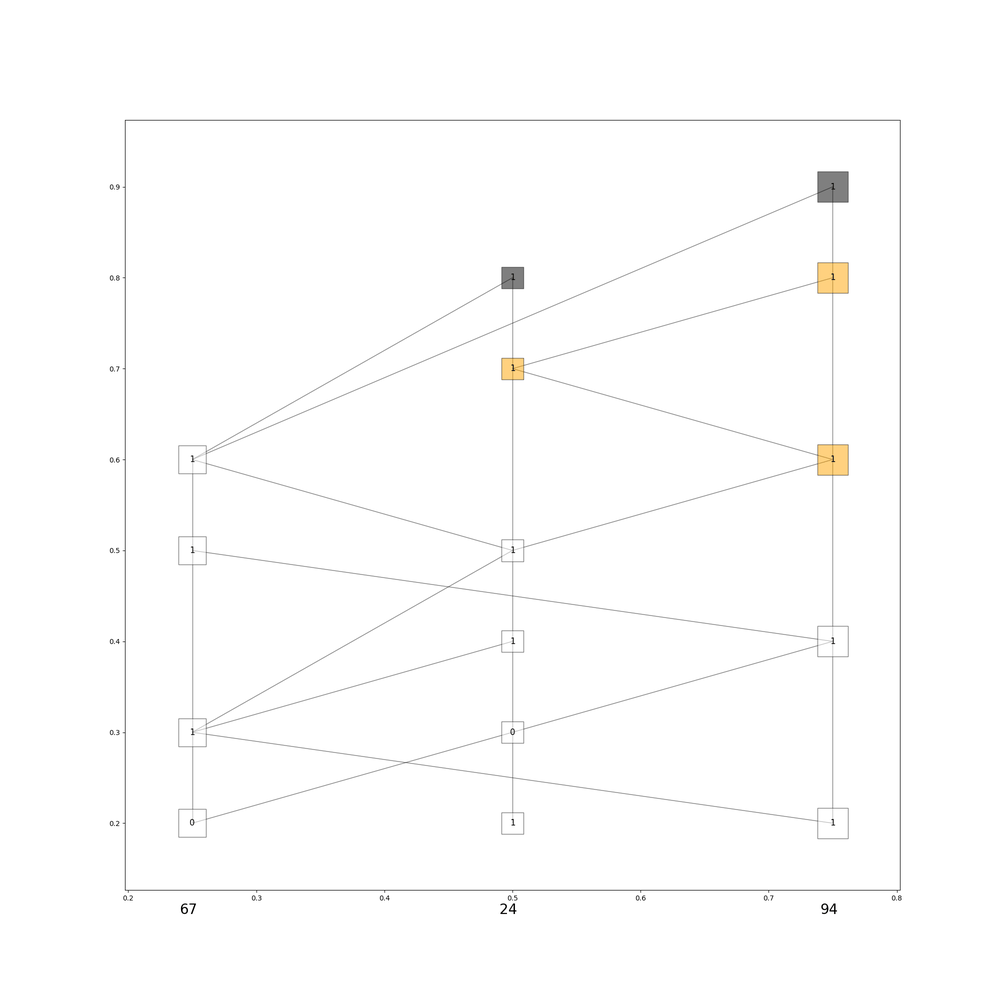
\includegraphics[width=0.5\textwidth]{3binary.png}
\caption{A Binary consensus protocol execution. Dotted lines are messages included in the justification of the later message. The label on the nodes represents the estimate of the message. A message is coloured if it has achieved some amount of Byzantine fault tolerant estimate safety, accoring to a clique oracle given its justification. The darker the colour, the more faults are tolerated by the estimate}
\end{figure}


\begin{figure}[h!]
\centering
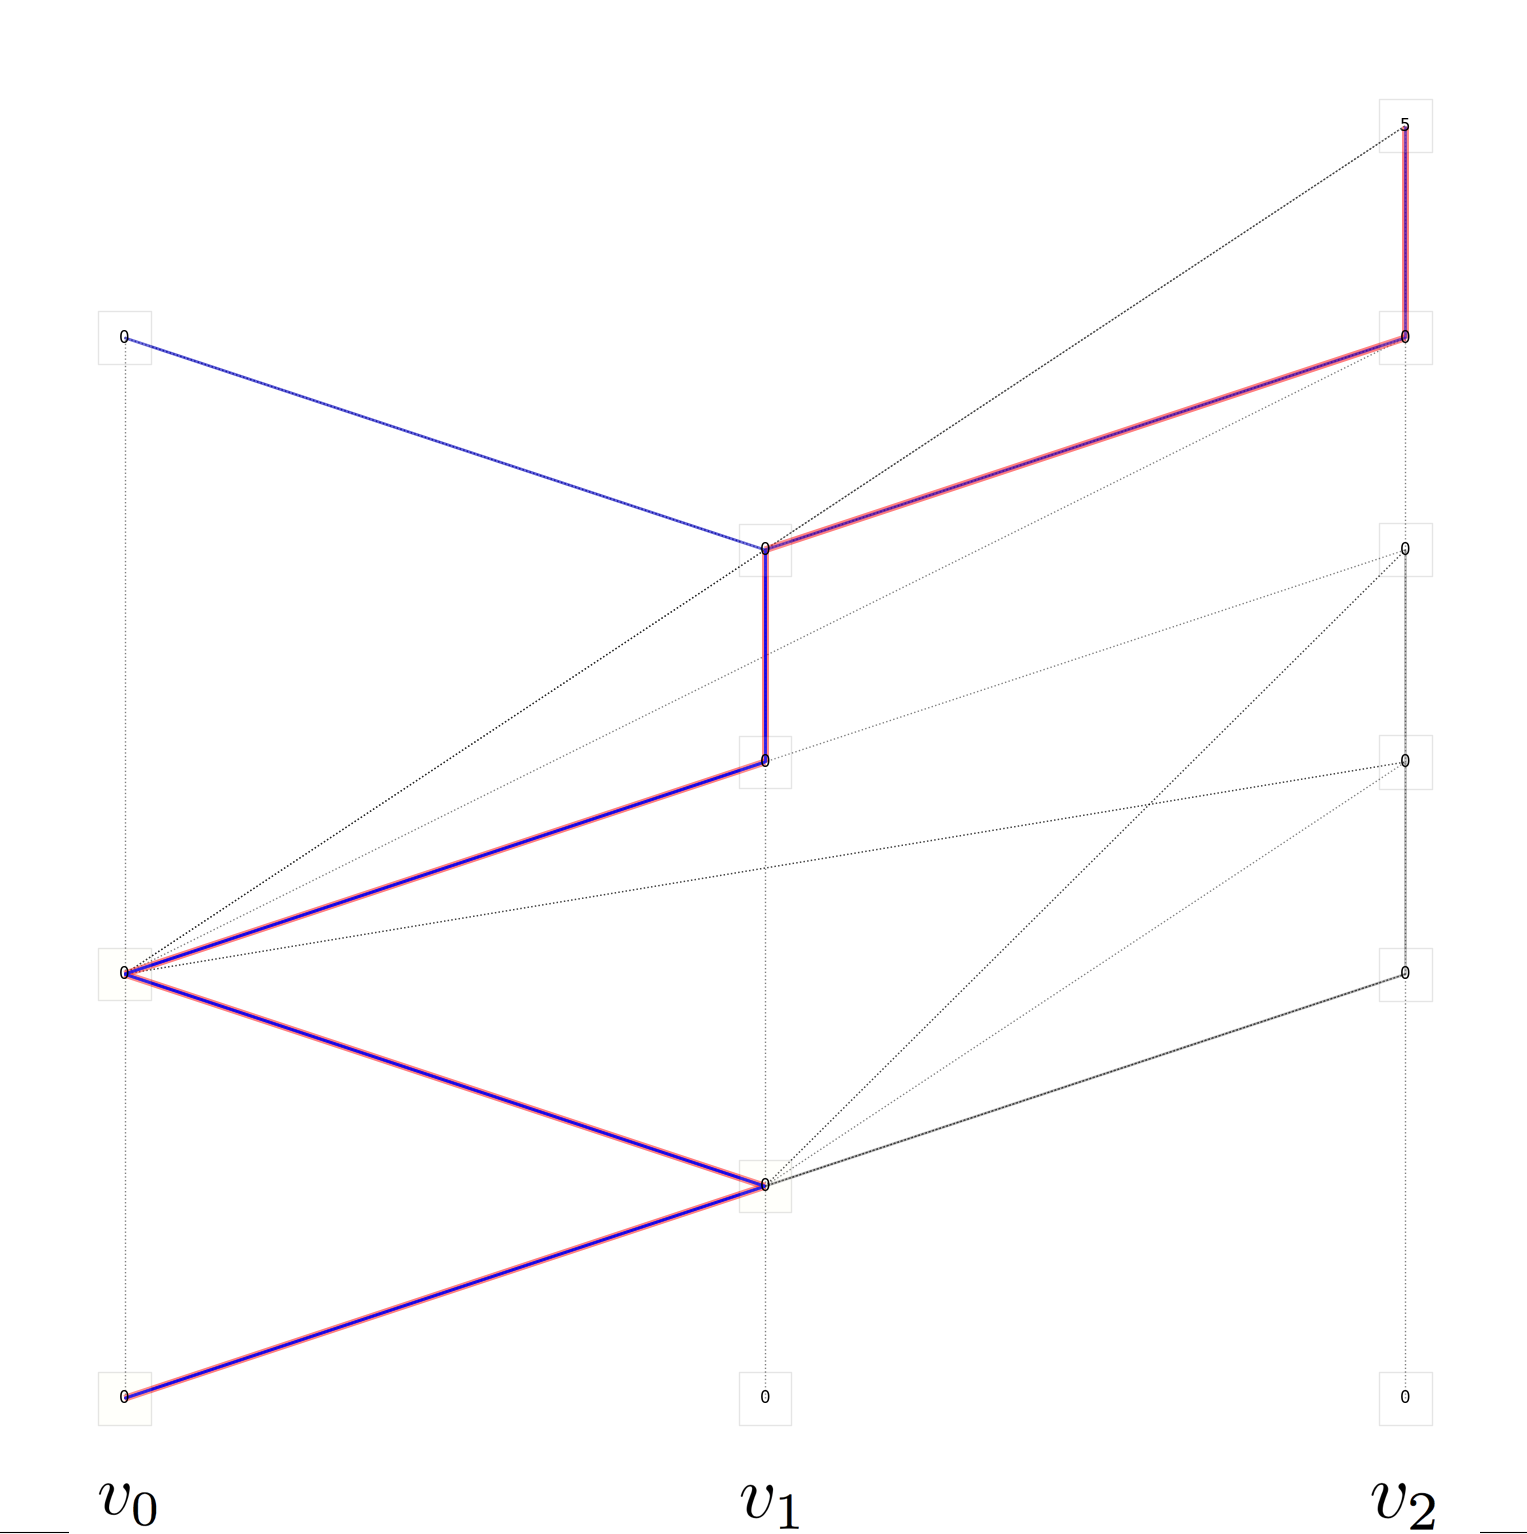
\includegraphics[width=0.5\textwidth]{3nodeblockchain.png}
\caption{Blockchain protocol execution with 3 validators, $v_0, v_1, v_2$. Each node labeled $0$ is the first message from that validator, and the nodes in the verical lines above each validator represent messages made by that validator. Dotted black lines are messages included in the justification of the later message. Blue lines represent the forkchoices of the validators given by their latest blocks. Solid grey lines prevblock pointers (that aren't blue because they are no longer the validator's forkchoice. The red line is the result of applying GHOST to the set of messages displayed here.}
\end{figure}


\begin{figure}[h!]
\centering
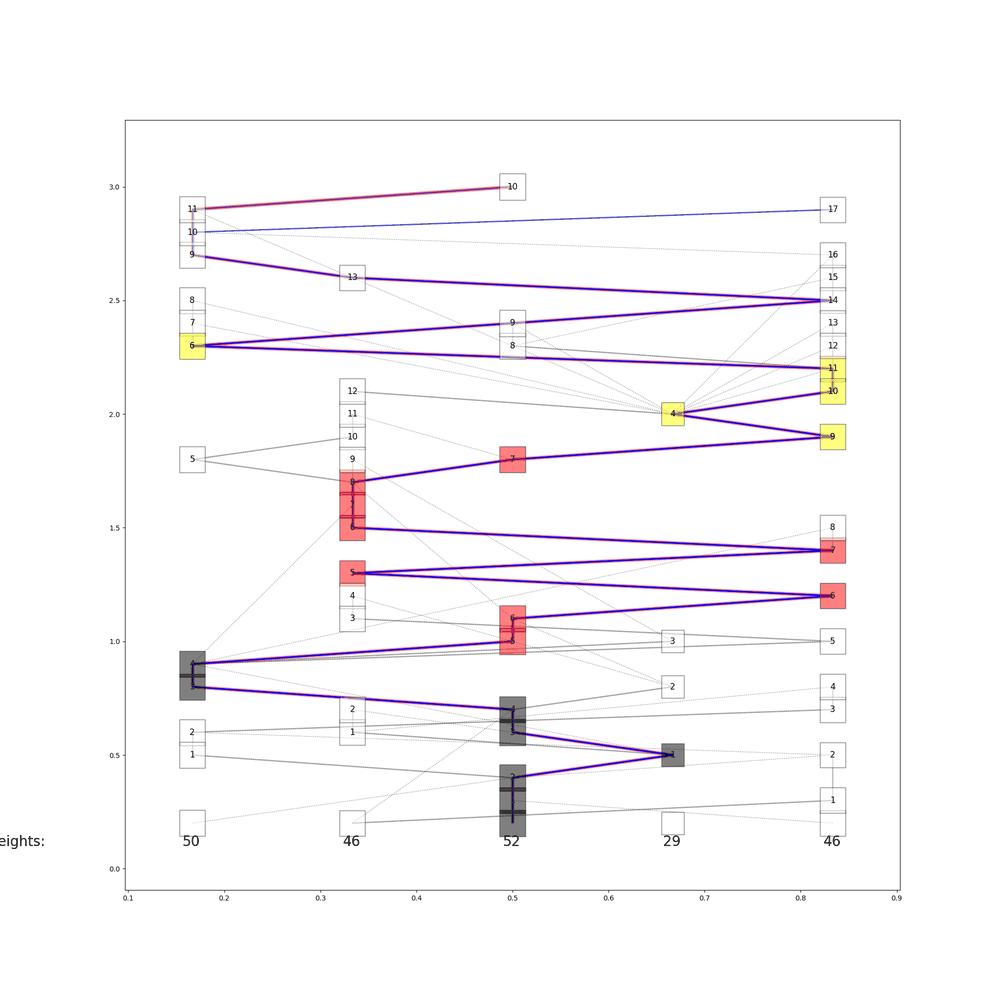
\includegraphics[width=0.5\textwidth]{blockchainsafety.png}
\caption{In this execution of the blockchain consensus protocol, we observe some safe blocks. They are colour coded the same way as in the earlier, however this time they represent the blocks that are seen to be safe from the view that includes all of the nodes. In contrast, in the binary consensus we displayed safety that was detected locally.}
\end{figure}


\begin{figure}[h!]
\centering
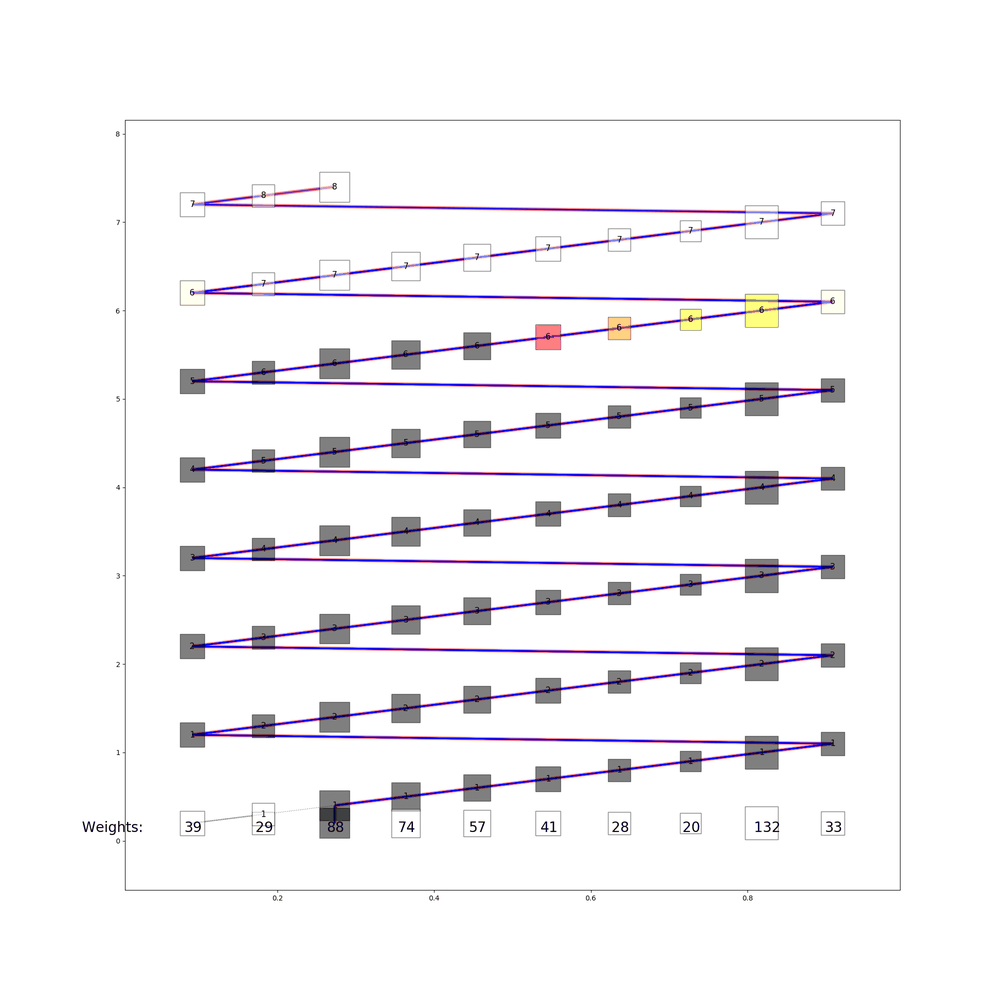
\includegraphics[width=0.5\textwidth]{roundrobin.png}
\caption{Finally, in this execution of the blockchain consensus protocol, where the validators are able to pass blocks around in a ``round-robin'' configuration, we observe the $\mathcal{O}(1)$ messages received per (finalized) block. This is possible because each block contributes to the consensus safety of many blocks.}
\end{figure}

\section{Conclusion}

We have given a brief overview of the consensus safety proof that Casper the Friendly Ghost has been derived to satisfy (in a ``correct-by-construction'' manner). Then we defined a binary consensus protocols (Casper the Friendly Binary Consensus) that satisfy the terms of the proof and therefore benefit from the results. We then remarkably slightly modified the binary consensus protocol to give the blockchain based consensus protocol (which can be adopted for, or even termed as sequential state machine replication). 

Then we further witnessed the power of the safety proof when we showed that we can remove the fault tolerance threshold from the protocol and do validator rotation without making significant changes to the protocol. Finally, we saw (as advertised) that it's possible for Casper the Friendly Ghost to decide on blocks with consensus safety that tolerates $t$ Byzantine faults (in an asynchronous network) with $\mathcal{O}(1)$ messages per block. 

We hope this work has been educational and will lead to the development of many interesting and useful consensus protocols.

\section{Acknowledgements}

I would like to thank Nate Rush and Danny Ryan for their hard work on getting the codebase ready for release at Devcon3, for their help on this (draft) paper. Thanks to Karl Floersch, who was the first developer to work on the codebase. I'd like to thank Greg Meredith for an introduction to the ``correct-by-construction'' approach to protocol design, as well as for helping formalize a lot of the ideas. Finally, I'd like to thank Vitalik Buterin, with whom I have collaborated on this research from its very early stages over three years ago.

\end{document}